\documentclass[11pt,a4paper]{article}

\usepackage[utf8]{inputenc}
\usepackage[T1]{fontenc}
\usepackage{lmodern}
\usepackage{graphicx}
\usepackage{booktabs}
\usepackage{amsmath}
\usepackage{hyperref}
\usepackage{natbib}
\usepackage[margin=2.5cm]{geometry}
\usepackage{xcolor}
\usepackage{float}
\usepackage{multirow}
\usepackage{array}
\usepackage{tabularx}
\usepackage{CJKutf8}

\bibliographystyle{plainnat}

\title{Excess Vocabulary in Japanese AI-Generated Text:\\A Cross-Model Quantitative Analysis}
\author{Ken Imoto\\Propel-lab\\Tokyo, Japan\\\texttt{imoto@propel-lab.co.jp}\\\url{https://kenimoto.dev}}
\date{March 2026}

\begin{document}
\begin{CJK}{UTF8}{min}

\maketitle

\begin{abstract}
We present the first quantitative analysis of excess vocabulary in Japanese AI-generated text. While prior work has identified characteristic ``slop words'' in English-language LLM outputs (e.g., \textit{delve}, \textit{intricate}), no equivalent study has been conducted for Japanese, a language with fundamentally different morphological structure. We generated 350 text samples across 7 LLMs---Claude 3 Haiku (\texttt{claude-3-haiku-20240307}), Claude Sonnet 4 (\texttt{claude-sonnet-4-20250514}), Claude Opus 4 (\texttt{claude-opus-4-20250514}), GPT-3.5 Turbo, GPT-4o, GPT-OSS 20B (Swallow), and Llama 3.2 1B---and compared them against a human baseline corpus of 977 articles from Qiita and Zenn (2020--2026). Using MeCab morphological analysis and $\chi^2$ tests with Bonferroni correction, we identified 651 statistically significant excess words. Three key findings emerge: (1)~Japanese excess vocabulary exhibits language-specific patterns distinct from English, with katakana loanwords and formal expressions predominating; (2)~newer Claude model generations show \emph{increasing} excess scores (mean excess: 60.1 $\to$ 74.4 $\to$ 105.0) alongside \emph{decreasing} lexical diversity (TTR: 0.52 $\to$ 0.32 $\to$ 0.29); and (3)~68\% of top AI excess words show increased frequency in post-LLM human articles (2024--2026), suggesting vocabulary coevolution between AI and human writers. We further validate these findings through four supplementary experiments: a control experiment against beginner and expert human writers (overlap with AI excess words $\leq$2.0\%), a cross-genre analysis on 270 documents across three genres demonstrating strong domain dependence (inter-genre Jaccard similarity = 0.00 with technical blogs), a classification experiment achieving in-domain AUC = 0.946 with complete cross-domain failure (AUC $\leq$ 0.535), confirming that excess vocabulary is inherently domain-bound, and semantic clustering via both t-SNE and hierarchical methods revealing interpretable groupings among the top 100 excess words.
\end{abstract}

\section{Introduction}

The rapid proliferation of Large Language Models (LLMs) has led to an unprecedented volume of AI-generated text across all domains, from academic papers to technical documentation and social media~\citep{openai2024gpt4, anthropic2025claude}. As AI-generated content becomes increasingly prevalent, the ability to distinguish it from human-written text has emerged as a critical challenge.

Recent research in English has identified characteristic vocabulary patterns---termed ``excess vocabulary'' or ``slop words''---that appear disproportionately in LLM-generated text compared to human writing~\citep{kobak2024vocabulary}. Words such as \textit{delve}, \textit{intricate}, \textit{commendable}, and \textit{pivotal} have been shown to occur at significantly elevated frequencies in AI outputs, serving as potential markers for AI text detection. Studies in the biomedical domain have further documented contamination of scientific literature with such excess vocabulary~\citep{liang2024monitoring, gray2024chatgpt}.

However, these findings are predominantly based on English-language corpora. Japanese, with its agglutinative morphology, three writing systems (hiragana, katakana, kanji), and distinct syntactic structure, presents fundamentally different challenges for excess vocabulary analysis. It remains an open question whether English-language findings regarding AI text characteristics transfer to Japanese, or whether Japanese AI-generated text exhibits its own language-specific excess patterns.

This paper makes the following contributions:
\begin{enumerate}
    \item The \textbf{first quantitative analysis} of excess vocabulary in Japanese AI-generated text, identifying 651 statistically significant excess words across 1,684 candidates.
    \item A \textbf{cross-model comparison} across 7 LLMs spanning commercial (Claude, GPT) and open-source (Swallow, Llama) models, revealing model-specific vocabulary signatures.
    \item A \textbf{generational analysis} of the Claude model family (Haiku $\to$ Sonnet 4 $\to$ Opus 4), demonstrating that newer generations exhibit higher excess scores and lower lexical diversity.
    \item A \textbf{cross-linguistic comparison} with English excess vocabulary, identifying shared patterns and language-specific divergences.
    \item A \textbf{coevolution analysis} comparing pre-LLM (2020--2022) and post-LLM (2024--2026) human articles, providing evidence that AI excess vocabulary is permeating human technical writing.
    \item A \textbf{control experiment} comparing AI excess words against beginner and expert human writers, demonstrating that excess vocabulary is AI-specific rather than an artifact of expository register.
    \item A \textbf{classification application} showing that excess word features achieve in-domain AUC = 0.946, with cross-domain evaluation revealing complete failure (AUC $\leq$ 0.535), establishing both practical utility and domain constraints.
    \item A \textbf{semantic clustering analysis} comparing t-SNE ($k$-means, $k=5$, silhouette = 0.128) and hierarchical clustering ($k=8$, silhouette = 0.140), with UMAP visualization confirming that excess vocabulary is organized by stylistic function rather than tight semantic categories.
\end{enumerate}

\section{Related Work}

\paragraph{Excess Vocabulary in English.}
\citet{kobak2024vocabulary} systematically identified words whose frequency increased sharply in AI-generated and AI-influenced English text, coining the term ``excess vocabulary.'' Their analysis revealed that words like \textit{delve}, \textit{intricate}, and \textit{commendable} appear at rates 2--10$\times$ higher in ChatGPT outputs compared to human baselines. \citet{liang2024monitoring} extended this to academic peer reviews, finding statistically significant vocabulary shifts in post-ChatGPT conference submissions. \citet{gray2024chatgpt} documented similar contamination in biomedical literature published in PubMed.

\paragraph{Human-LLM Coevolution.}
\citet{arrigo2025coevolution} investigated the bidirectional influence between LLM outputs and human writing, finding evidence that human academic writing has begun adopting stylistic features characteristic of LLM-generated text. This coevolution phenomenon raises concerns about the long-term homogenization of written language.

\paragraph{LLM Behavioral Patterns.}
\citet{malmqvist2024sycophancy} analyzed sycophantic tendencies in LLMs, demonstrating that instruction-tuned models tend to produce overly positive, emphatic, and verbose responses. This behavioral pattern is closely related to excess vocabulary, as sycophantic tendencies may drive the overuse of emphatic and formal expressions.

\paragraph{Japanese NLP and Stylometry.}
Research on Japanese stylometry has recently extended to AI-generated text detection. \citet{zaitsu2023chatgpt} conducted the first stylometric analysis distinguishing ChatGPT-3.5 and ChatGPT-4 generated Japanese text from human writing, demonstrating that statistical features such as sentence length distribution, character type ratios, and vocabulary richness can effectively separate AI from human authorship. In a follow-up study, \citet{zaitsu2025stylometry} expanded this analysis to seven LLMs, finding that stylometric methods achieve high classification accuracy while human judges struggle to distinguish AI-generated Japanese text. \citet{kanda2025ensemble} developed an integrated ensemble of BERT-based and feature-based models for authorship attribution in Japanese literary works, achieving F1 scores above 0.96 even for short text segments of 510 tokens. On the detection methodology side, \citet{koike2024outfox} proposed OUTFOX, an in-context learning approach for LLM-generated essay detection using adversarially generated examples, presented at AAAI 2024. For corpus-level analysis of Japanese register variation, the Balanced Corpus of Contemporary Written Japanese (BCCWJ)~\citep{maekawa2014bccwj} provides a 100-million-word reference corpus spanning multiple registers, enabling systematic comparison of vocabulary distributions across genres. Our work complements these studies by focusing specifically on \emph{lexical} excess patterns rather than stylometric features, and by analyzing cross-model and cross-generational variation.

\paragraph{AI Text Structural Analysis.}
In our prior work~\citep{imoto2025slop}, we identified 16 structural patterns characteristic of AI-generated text (``AI Text Slop''), including excessive use of bullet points, formulaic transitions, and hedging language. The present study extends this line of research by focusing specifically on lexical excess at the morpheme level in Japanese.

\section{Methodology}

\subsection{AI Text Generation}

We generated text samples using 7 LLMs representing diverse architectures, scales, and training paradigms:

\begin{itemize}
    \item \textbf{Claude family} (Anthropic): Claude 3 Haiku, Claude Sonnet 4, Claude Opus 4
    \item \textbf{GPT family} (OpenAI): GPT-3.5-turbo, GPT-4o
    \item \textbf{Open-source}: GPT-OSS 20B (Swallow), Llama 3.2 1B (Meta)
\end{itemize}

For each model, we prepared 10 technical blog themes in Japanese covering topics such as Python exception handling, Docker containerization, database design, CI/CD pipelines, web security, Git workflow, REST API design, code review practices, agile development, and infrastructure as code. Each theme was generated 5 times per model using a unified prompt template, yielding $7 \times 10 \times 5 = 350$ samples. All generations used default temperature settings to reflect typical usage conditions.

\subsection{Human Corpus Collection}

The human baseline corpus was collected from two major Japanese technical blogging platforms: Qiita and Zenn. We assembled two temporal subcorpora:

\begin{itemize}
    \item \textbf{Pre-LLM corpus} (2020--2022): 700 articles, 573,279 tokens. Published before the widespread availability of ChatGPT (released November 2022), minimizing potential AI contamination.
    \item \textbf{Post-LLM corpus} (2024--2026): 277 articles, 237,954 tokens. Published after LLMs became widely accessible, enabling coevolution analysis.
\end{itemize}

The total human corpus comprises 977 articles. The pre-LLM subcorpus served as the primary human baseline for excess score computation.

\subsection{Morphological Analysis}

Japanese text requires morphological analysis for tokenization, as the language does not use whitespace to delimit words. We employed MeCab~\citep{kudo2006mecab} with the UniDic-lite dictionary~\citep{unidic2021} for morphological segmentation and lemmatization (extraction of dictionary base forms, 原形). This approach normalizes inflected forms to their canonical representations, enabling consistent frequency comparison across corpora.

From the tokenized output, we extracted:
\begin{itemize}
    \item \textbf{Word frequencies}: Normalized occurrence rates per token for each word.
    \item \textbf{N-gram frequencies}: Bigram and trigram patterns at the morpheme level.
    \item \textbf{Sentence-initial patterns}: First morpheme of each sentence, capturing discourse-level tendencies.
\end{itemize}

\subsection{Excess Score Calculation}

Following \citet{kobak2024vocabulary}, we define the \textit{excess score} of a word $w$ as:

\begin{equation}
    \text{excess\_score}(w) = \frac{f_{\text{AI}}(w) - f_{\text{human}}(w)}{f_{\text{human}}(w)}
\end{equation}

\noindent where $f_{\text{AI}}(w)$ and $f_{\text{human}}(w)$ denote the normalized frequency (occurrences per total tokens) of word $w$ in the AI-generated and human corpora, respectively. An excess score of $+10$ indicates that the word appears $11\times$ more frequently in AI text than in human text.

Statistical significance was assessed using the $\chi^2$ test for each word's contingency table (AI count vs.\ human count, adjusted for corpus size). We applied Bonferroni correction for multiple comparisons across all 1,684 tested words, using a family-wise significance threshold of $\alpha = 0.05$.

To quantify the practical magnitude of frequency differences beyond statistical significance, we computed Cohen's $d$ effect size for each excess word. For each word $w$, we obtained per-model normalized frequencies across the 7 AI models and compared them against the human baseline frequency, yielding an effect size estimate that is robust to corpus size inflation of $\chi^2$ statistics. Following standard conventions, we classify $|d| \geq 0.8$ as large, $0.5 \leq |d| < 0.8$ as medium, and $0.2 \leq |d| < 0.5$ as small effects.

For cross-model comparison, we computed per-model excess scores using each model's generated corpus against the shared human baseline. Inter-model distributional differences were assessed using the Mann-Whitney $U$ test with Bonferroni correction across all pairwise comparisons.

\section{Results}

\subsection{Japanese Excess Words}

Our analysis identified 1,684 candidate excess words across the combined AI corpus. Of these, 1,124 were statistically significant at $p < 0.05$ without correction, and \textbf{651 remained significant after Bonferroni correction} ($p < 0.05 / 1{,}684$). Table~\ref{tab:top20} presents the top 20 excess words ranked by excess score.

\begin{table}[H]
\centering
\caption{Top 20 Japanese excess words with statistical significance (Bonferroni-corrected).}
\label{tab:top20}
\small
\begin{tabular}{rlrrrr}
\toprule
Rank & Word & Excess Score & $\chi^2$ & AI Count & Human Count \\
\midrule
1  & Hash              & +189.08 & 1,830.73 & 402 & 10 \\
2  & Parent            & +176.96 & 1,881.11 & 414 & 11 \\
3  & レート (rate)      & +172.06 & 3,328.34 & 732 & 20 \\
4  & Review            & +169.65 & 1,800.72 & 397 & 11 \\
5  & カスケード (cascade) & +161.34 & 1,397.39 & 309 & 9 \\
6  & Image             & +107.38 & 3,873.37 & 871 & 38 \\
7  & Tool              & +67.56  & 119.34   & 29  & 2 \\
8  & NF                & +62.83  & 340.31   & 81  & 6 \\
9  & Travis            & +62.83  & 109.98   & 27  & 2 \\
10 & deployment        & +60.47  & 160.53   & 39  & 3 \\
11 & バージョニング & +56.69 & 252.26 & 61 & 5 \\
12 & エスケープ (escape) & +53.85 & 238.23 & 58 & 5 \\
13 & XSS               & +50.42  & 357.14   & 87  & 8 \\
14 & スクリプティング & +49.44 & 127.83 & 32 & 3 \\
15 & development       & +47.23  & 205.54   & 51  & 5 \\
16 & 立案  & +46.28  & 118.52   & 30  & 3 \\
17 & クロスサイトリクエストフォージェリ & +46.28 & 77.36 & 20 & 2 \\
18 & Found             & +43.92  & 72.72    & 19  & 2 \\
19 & こつ  & +41.56  & 396.77   & 99  & 11 \\
20 & CSRF              & +41.56  & 323.71   & 81  & 9 \\
\bottomrule
\end{tabular}
\end{table}

Additionally, we identified \textbf{104 AI-only words}---words that appeared in AI-generated text but had zero occurrences in the human corpus. Notable examples include ``Automated'' (116 occurrences), 脆い (\textit{moroi}, ``fragile,'' 70 occurrences), リダイレクション (``redirection,'' 42 occurrences), and ``Dockerized'' (38 occurrences).

\paragraph{AI-Only Word Analysis.}
The 104 AI-only words exhibit a distinctive script distribution: 67 (64.4\%) are English/ASCII terms, 10 (9.6\%) are katakana, 18 (17.3\%) are kanji compounds, and 9 (8.7\%) are mixed-script tokens. The overwhelming dominance of English terms suggests that LLMs default to source-language technical vocabulary where human writers would use Japanese alternatives or avoid the term entirely.

Model-wise, Llama~3.2~1B contributed the most AI-only words (65 of 104, with 58 exclusive to Llama), reflecting its limited parameter count and resulting in code-mixed outputs including Chinese characters (码检, 查看) and malformed tokens (uthentication). Only 19 AI-only words were used by 3 or more models, including technically specific terms such as プリペアドステートメント (``prepared statement,'' used by 6 models), SonarQube, and dockerignore.

The prevalence of AI-only words raises the question of \emph{why} LLMs generate words absent from human technical writing. Three hypotheses are plausible: (1)~\textbf{training data leakage}: models reproduce English-dominant documentation verbatim rather than adapting to Japanese conventions; (2)~\textbf{over-specification}: instruction-tuned models attempt to demonstrate comprehensive knowledge by using precise technical terms that human writers would paraphrase or omit; and (3)~\textbf{tokenization artifacts}: subword tokenization during training creates spurious morpheme boundaries, producing tokens like ``コンポジット-composite'' that reflect BPE segmentation rather than natural Japanese usage.

Figure~\ref{fig:excess_words} visualizes the distribution of excess scores for the top 30 words, and Figure~\ref{fig:excess_ngrams} shows the top 20 excess n-grams. The highest-scoring n-gram was ``Python 例外 処理'' (``Python exception handling,'' excess score +224.35), indicating that AI models tend to use highly formulaic multi-word expressions.

\begin{figure}[H]
\centering
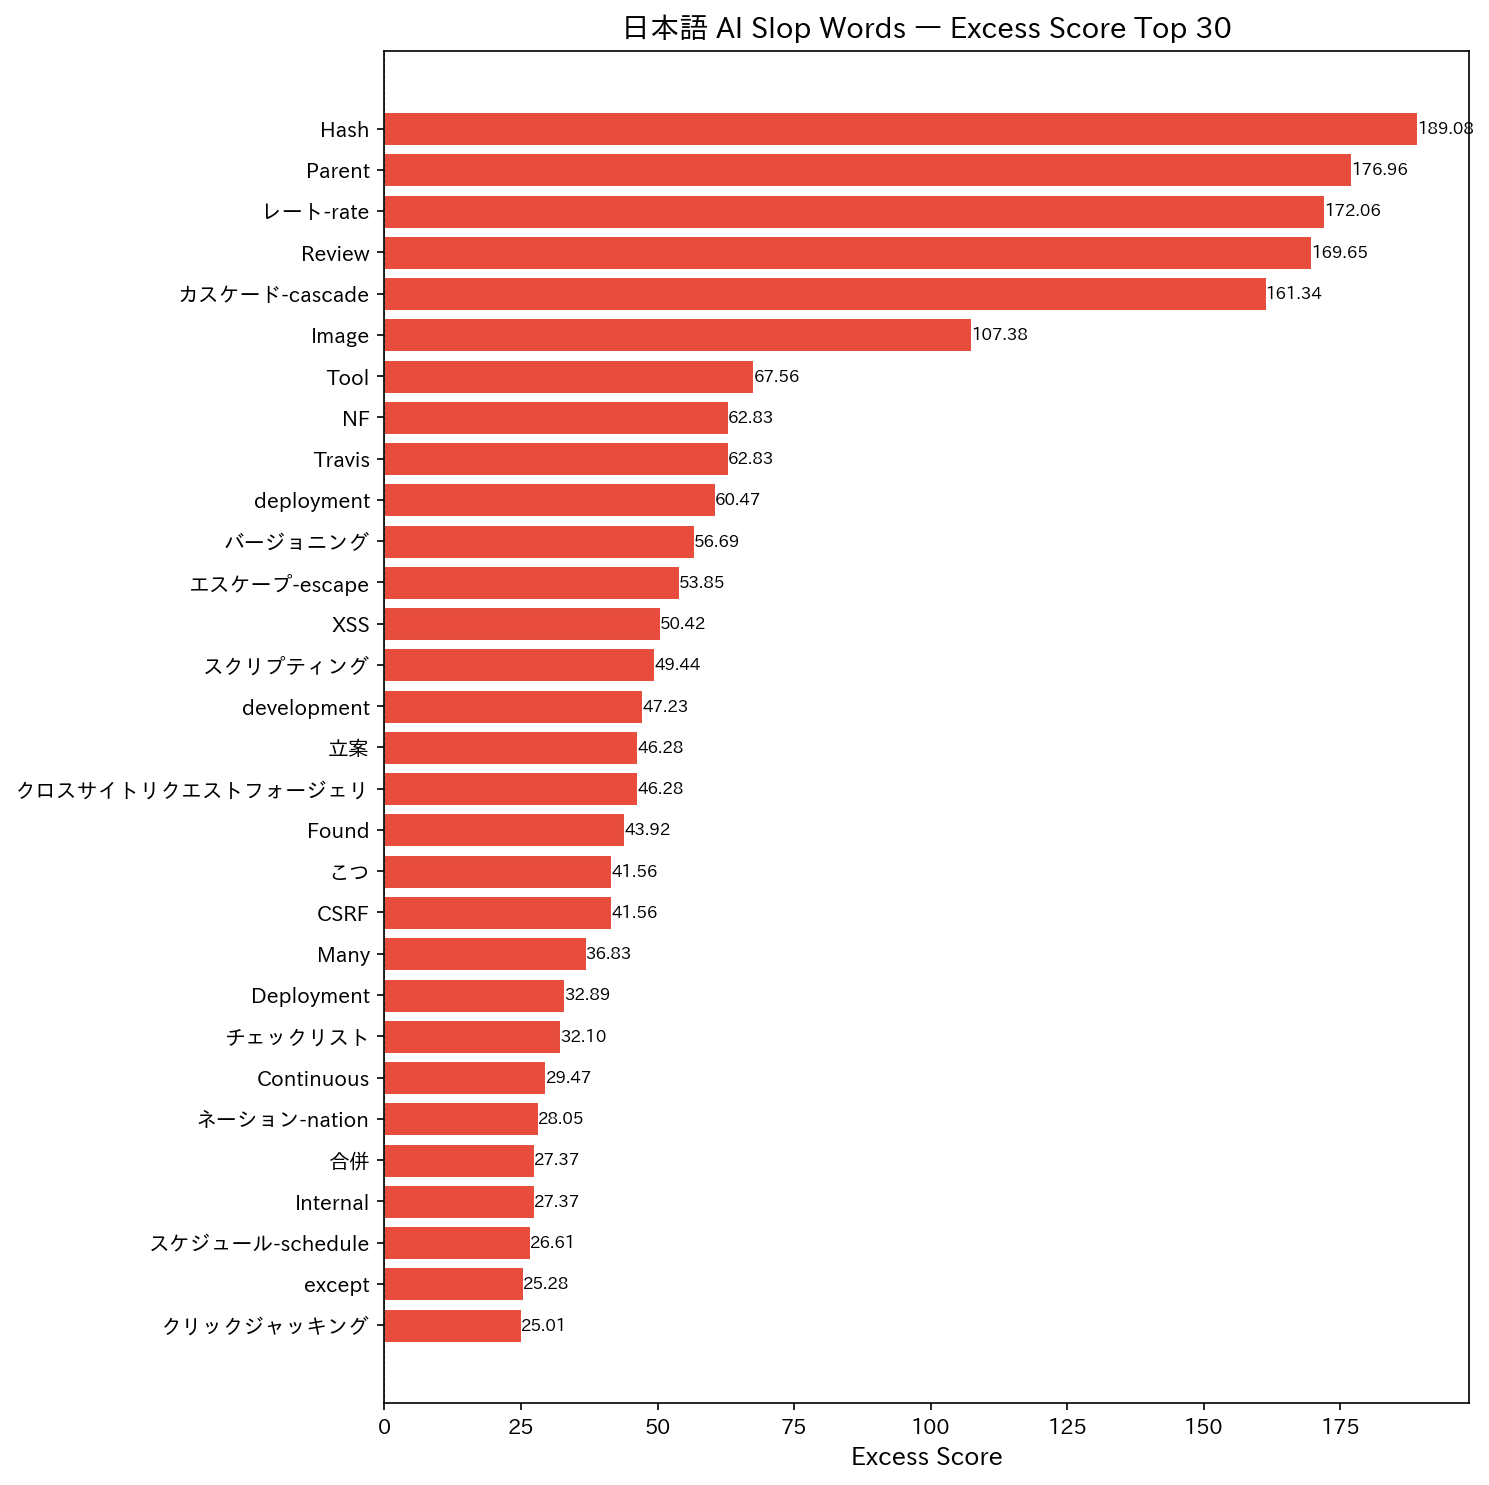
\includegraphics[width=0.85\textwidth]{../results/figures/excess_words_top30.png}
\caption{Top 30 Japanese excess words ranked by excess score. The horizontal axis shows the excess score (ratio of AI--human frequency difference to human frequency), while bars represent individual words. Words at the top (Hash, Parent, レート) exhibit AI frequencies over 170$\times$ their human baseline. The dominance of English loanwords and katakana technical terms is visually apparent, reflecting LLMs' preference for formal, internationalized vocabulary.}
\label{fig:excess_words}
\end{figure}

\begin{figure}[H]
\centering
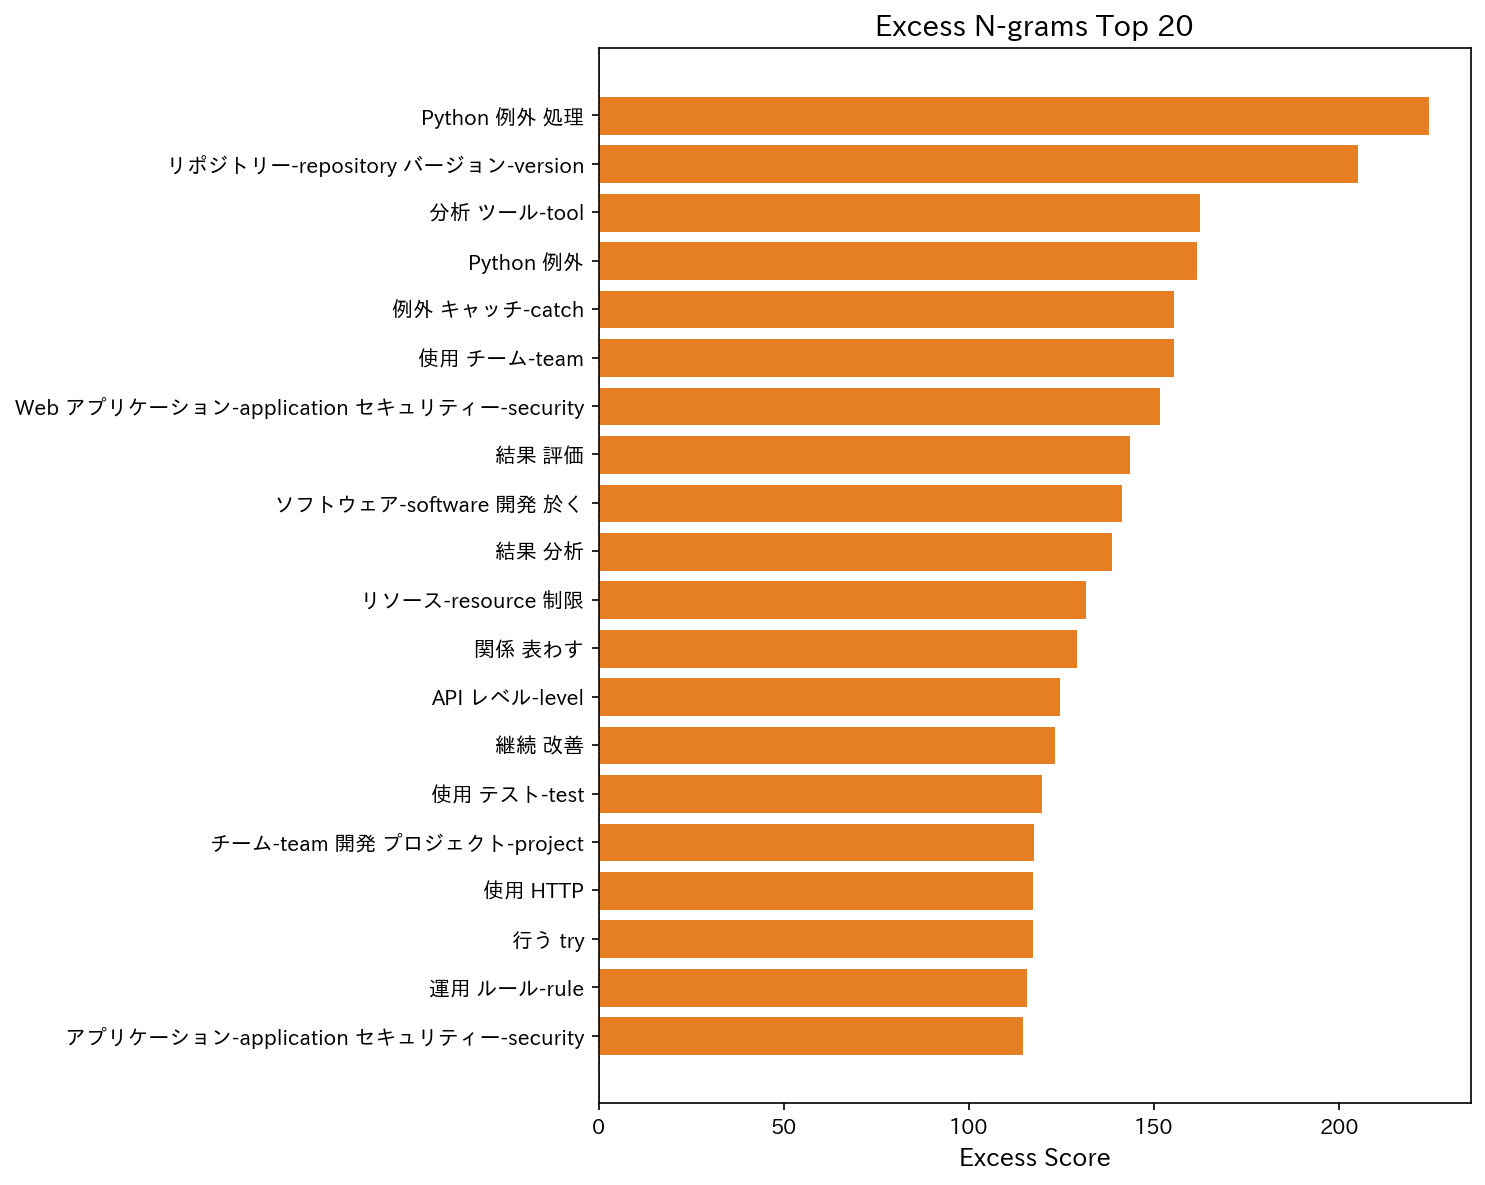
\includegraphics[width=0.85\textwidth]{../results/figures/excess_ngrams_top20.png}
\caption{Top 20 excess n-grams (morpheme-level bigrams and trigrams). The highest-scoring n-gram ``Python 例外 処理'' (+224.35) reflects AI models' tendency to produce formulaic multi-word technical expressions. The prevalence of trigrams combining a technology name with an action concept (e.g., ``Docker コンテナ 化'') indicates that AI text over-relies on canonical phrasings rather than the varied expressions found in human writing.}
\label{fig:excess_ngrams}
\end{figure}

Sentence-initial excess analysis (Figure~\ref{fig:sentence_starters}) revealed that AI models disproportionately begin sentences with ``try'' (excess score +114.57), ``Code'' (+103.46), and 適切 (\textit{tekisetsu}, ``appropriate,'' +25.92). The prominence of 適切 and 主要 (\textit{shuyou}, ``primary,'' +22.71) as sentence starters reflects the tendency of LLMs to employ formal, evaluative language at the discourse level.

\begin{figure}[H]
\centering
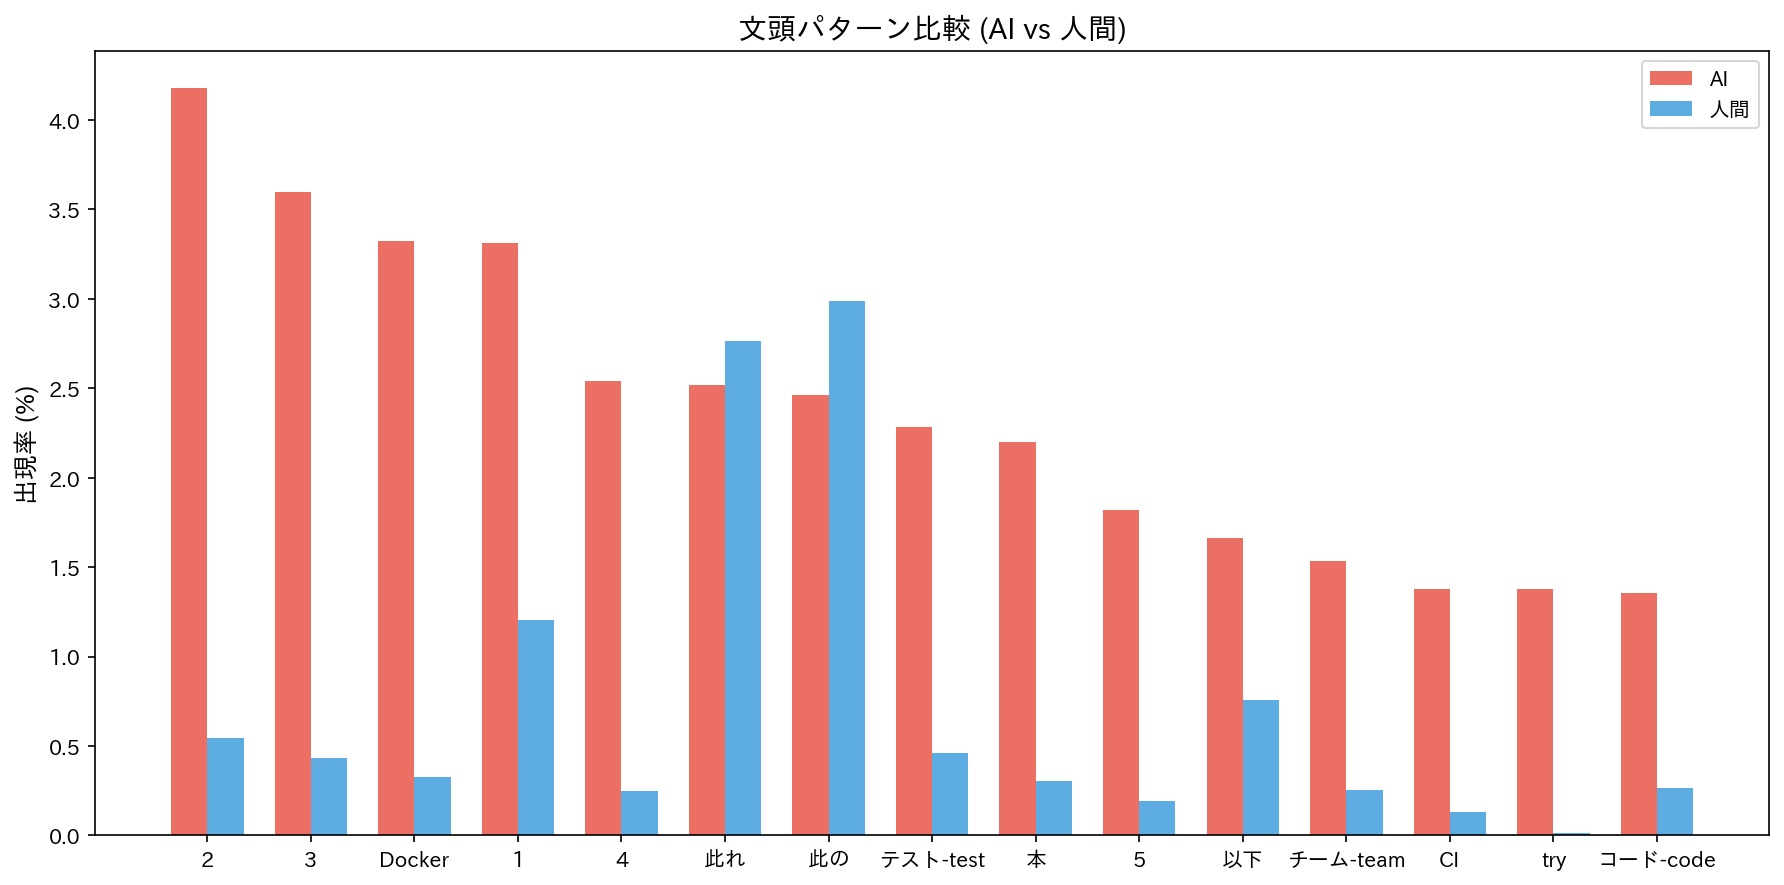
\includegraphics[width=0.85\textwidth]{../results/figures/sentence_starters.png}
\caption{Top 15 excess sentence-initial words. AI models disproportionately begin sentences with imperative/instructional words (``try,'' ``Code'') and formal evaluative adjectives (適切, 主要), reflecting a pedagogical, authoritative tone characteristic of instruction-tuned LLMs.}
\label{fig:sentence_starters}
\end{figure}

\subsection{Cross-Model Comparison}

Figure~\ref{fig:heatmap} presents a heatmap of model-specific excess scores for key vocabulary items. Several patterns emerge from the cross-model analysis.

\begin{figure}[H]
\centering
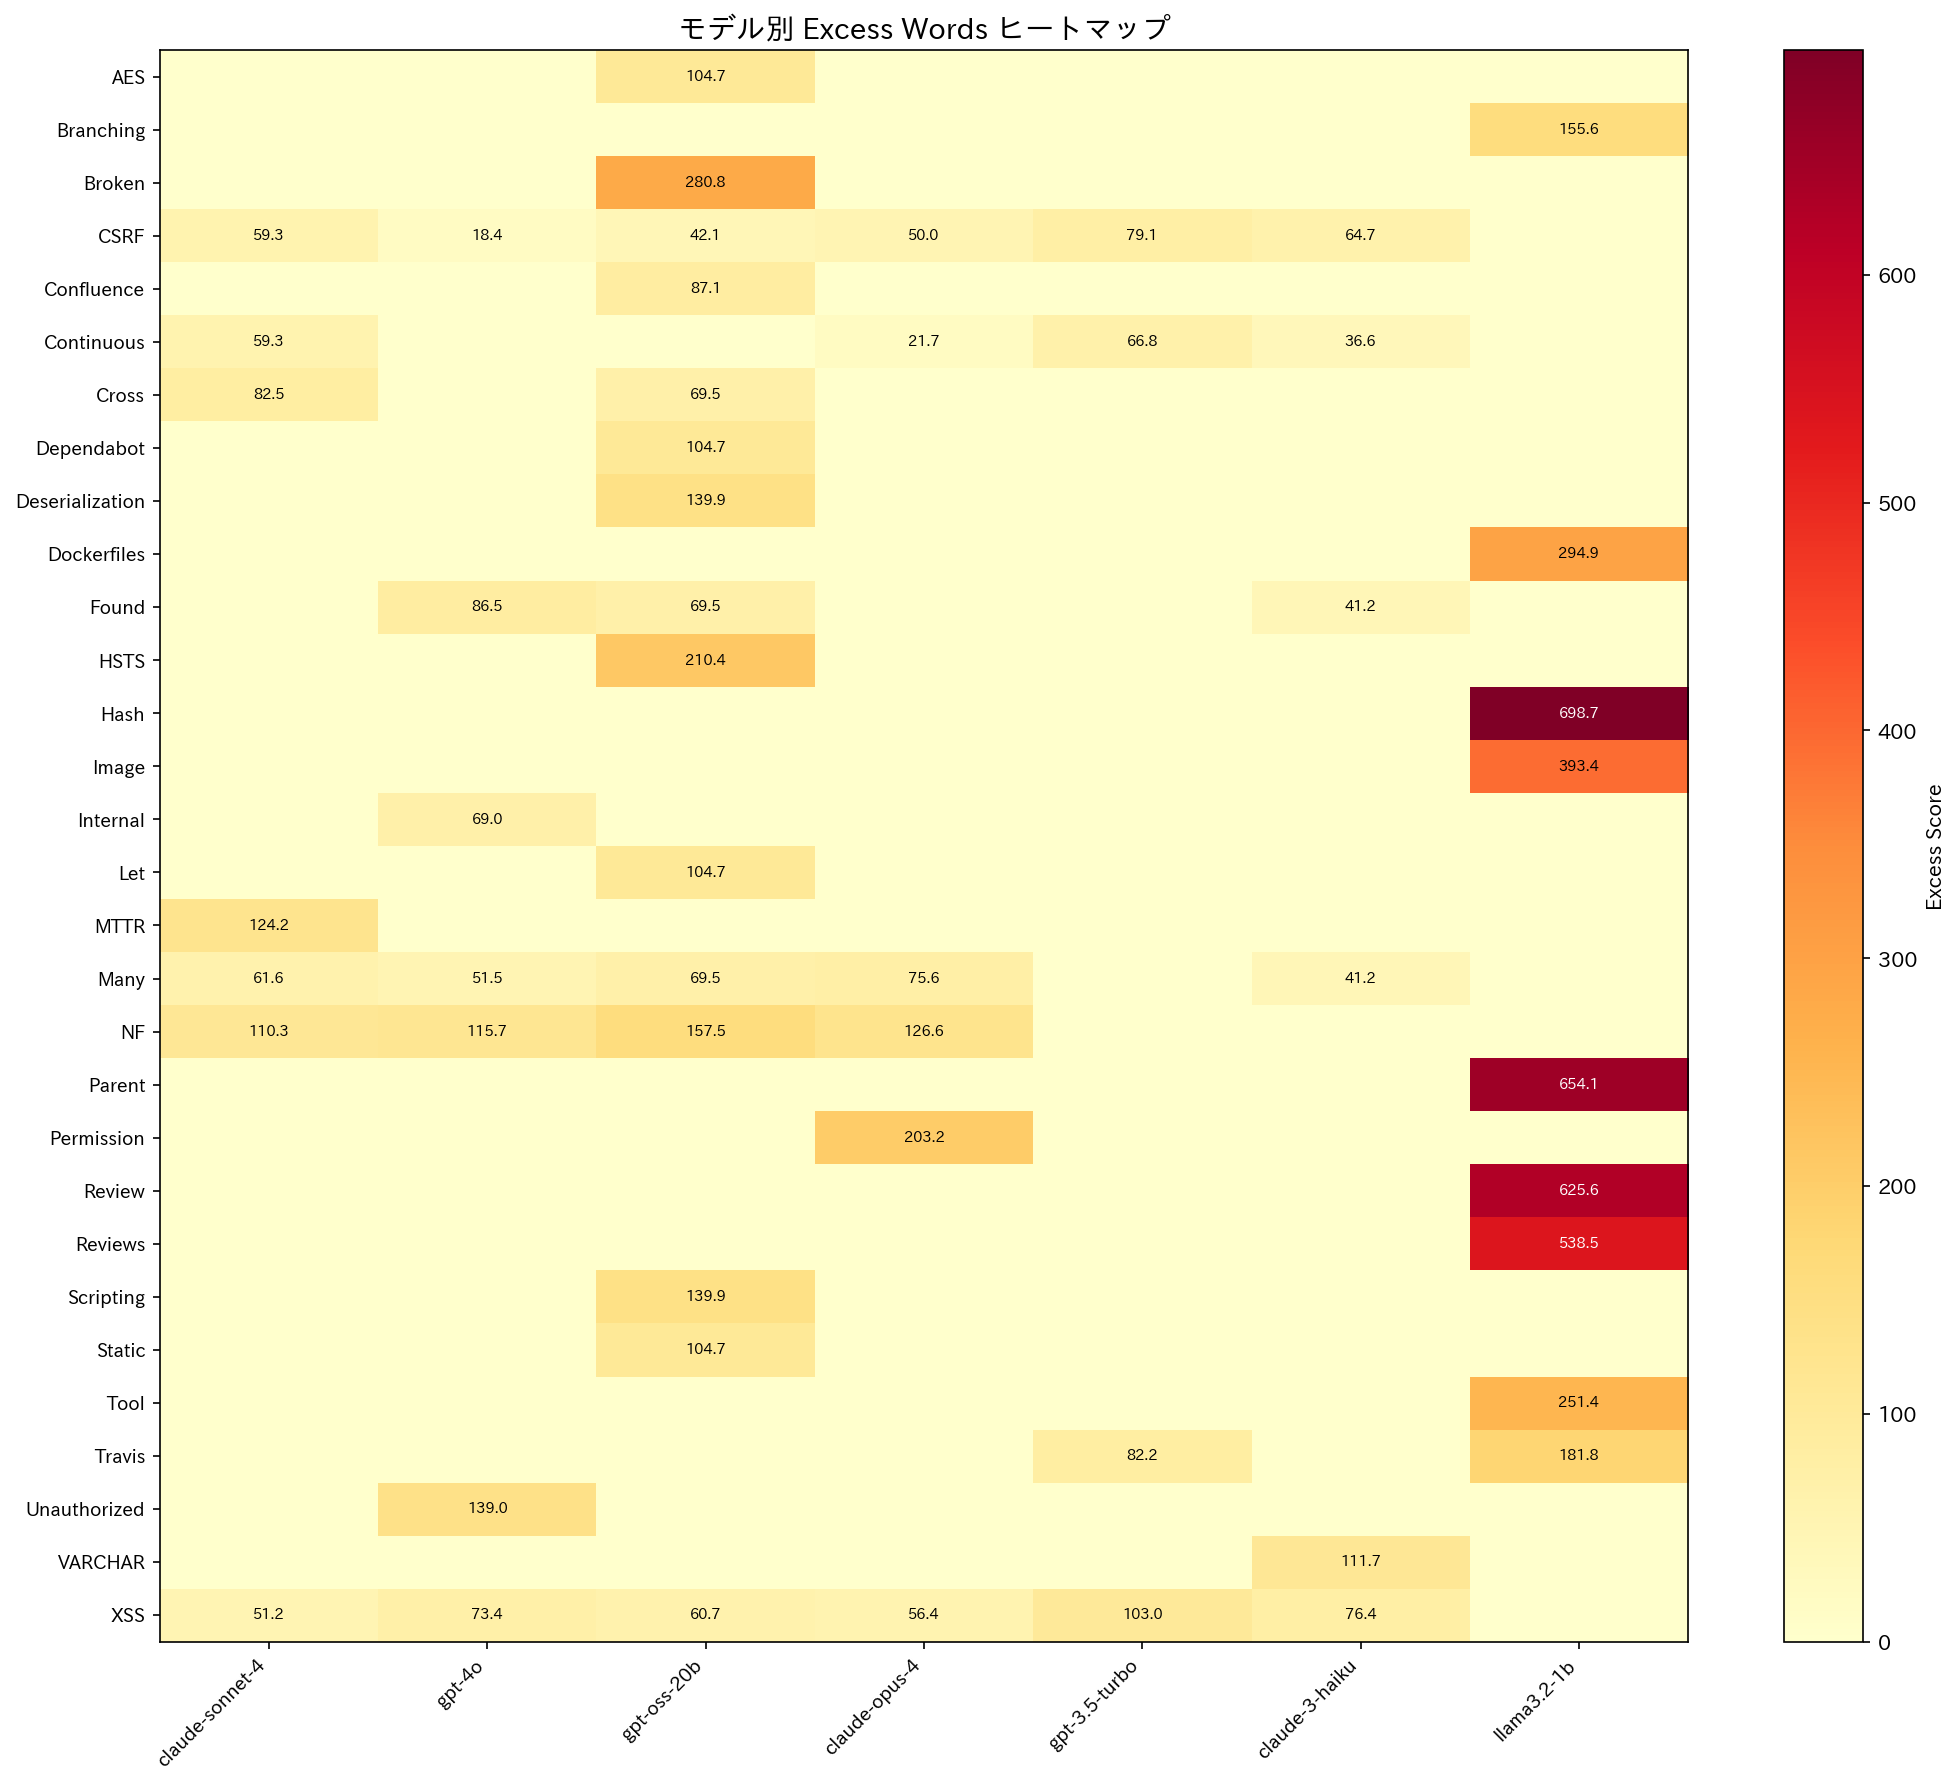
\includegraphics[width=0.95\textwidth]{../results/figures/model_heatmap.png}
\caption{Model-specific excess score heatmap across selected vocabulary items. Rows represent individual LLMs and columns represent excess words. Color intensity encodes the per-model excess score: darker cells indicate higher overuse relative to the human baseline, while white cells indicate absence or near-human-level frequency. Several patterns are notable: (1)~Llama~3.2~1B exhibits extreme scores concentrated in a narrow set of words (Hash: +698.67, Parent: +654.05), reflecting the 1B-parameter model's limited vocabulary distribution and heavy lexical repetition; (2)~Claude generations show a progressive broadening of moderate-to-high excess cells from Haiku to Opus~4, consistent with the generational excess escalation reported in Section~4.3; (3)~GPT-OSS~20B (Swallow) displays a distinctive column pattern in domain-specific terms (e.g., ページング, Broken) absent from other models, likely artifacts of Japanese-specific fine-tuning; (4)~GPT-4o shows comparatively sparse excess, with its strongest signals in specialized vocabulary (原子: +174.05).}
\label{fig:heatmap}
\end{figure}

\paragraph{Llama 3.2 1B (open-source, small).}
This model exhibited the most extreme individual excess scores, with ``Hash'' (+698.67), ``Parent'' (+654.05), and ``Review'' (+625.57). As the smallest model in our study (1B parameters), its limited vocabulary distribution leads to heavy repetition of specific terms.

\paragraph{GPT-OSS 20B (Swallow).}
The open-source Japanese-tuned model showed distinctive patterns including ページング (``paging,'' +457.00) and ``Broken'' (+280.85), suggesting that domain-specific fine-tuning can introduce unique vocabulary biases.

\paragraph{Commercial models (Claude, GPT).}
Claude and GPT models exhibited more moderate but consistent excess patterns. GPT-3.5-turbo showed high excess in security-related terminology (クリックジャッキング, +137.62; クロスサイトリクエストフォージェリ, +109.90), while GPT-4o favored 原子 (\textit{genshi}, ``atomic,'' +174.05).

\paragraph{Mann-Whitney $U$ test results.}
Pairwise comparison of excess score distributions revealed that Claude 3 Haiku had a significantly lower median excess score (0.94) than Claude Opus 4 (1.65, $p < 0.001$), Claude Sonnet 4 (1.41, $p < 0.01$), GPT-3.5-turbo (1.41, $p < 0.001$), and GPT-OSS 20B (1.44, $p < 0.001$). GPT-4o (median 1.04) also showed significantly lower excess than Claude Opus 4 ($p < 0.01$). These results suggest that model scale and instruction tuning intensity are associated with higher excess vocabulary.

\paragraph{Effect sizes (Cohen's $d$).}
Of the top 200 excess words analyzed for effect size, 126 (63.0\%) exhibited large effects ($|d| \geq 0.8$), 42 (21.0\%) medium effects, and 32 (16.0\%) small effects. The largest effect sizes were observed for topic-anchored words that appear consistently across all AI models: CD ($d = 6.79$), 例外 (``exception,'' $d = 6.19$), CI ($d = 4.50$), and こつ (``knack/tip,'' $d = 3.96$). Notably, the words with the highest \emph{excess scores} (Hash, Parent, レート) did not always show the largest Cohen's $d$ values, because their extreme frequencies are driven by a single model (Llama~3.2) rather than being consistent across all models. This dissociation between excess score and effect size underscores the importance of reporting both metrics: excess score captures the maximum AI--human divergence, while Cohen's $d$ captures the consistency of that divergence across models.

\subsection{Generational Analysis (Claude)}

The Claude model family provides a natural experiment for examining how excess vocabulary evolves across model generations. Figure~\ref{fig:evolution} summarizes the generational trends.

\begin{figure}[H]
\centering
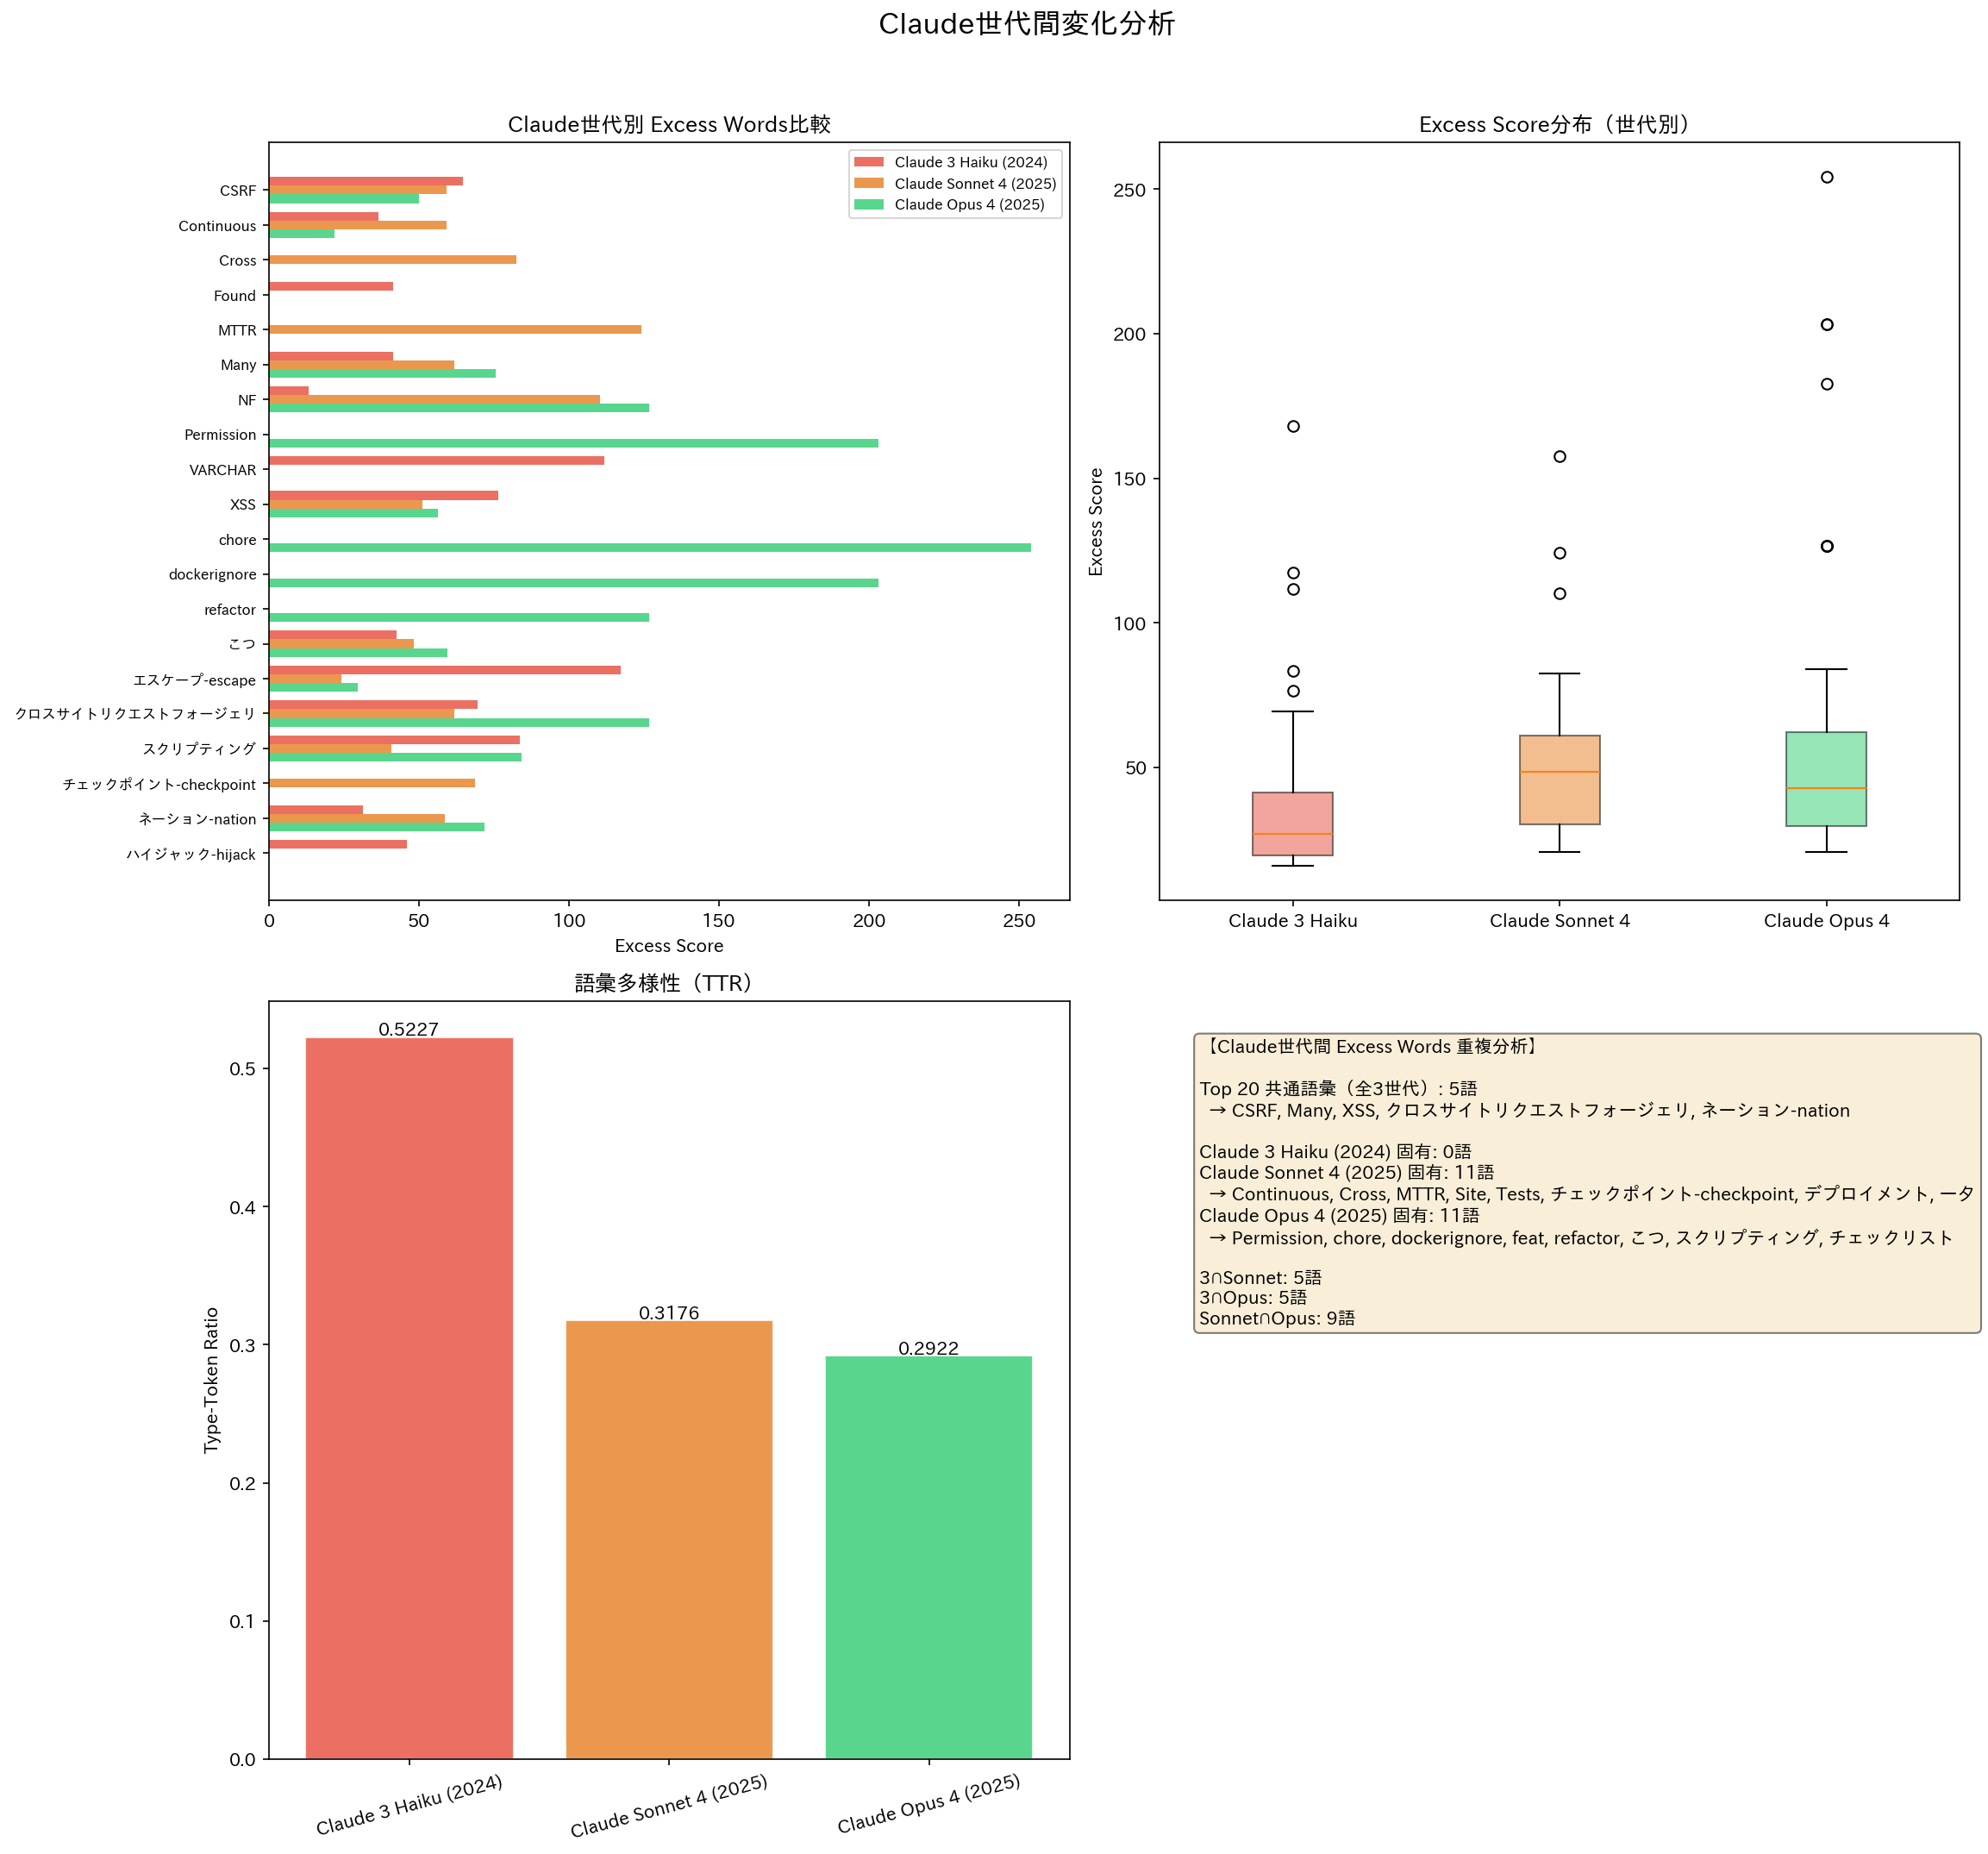
\includegraphics[width=0.85\textwidth]{../results/figures/model_evolution.png}
\caption{Claude generational evolution: excess scores and lexical diversity. The left panel shows increasing mean excess scores across Claude generations (Haiku~60.1 $\to$ Sonnet~4~74.4 $\to$ Opus~4~105.0), while the right panel shows monotonically declining Type-Token Ratio (0.52 $\to$ 0.32 $\to$ 0.29). This inverse relationship---greater capability accompanied by narrower vocabulary---suggests that RLHF and instruction tuning amplify lexical preferences at the expense of diversity.}
\label{fig:evolution}
\end{figure}

\paragraph{Lexical diversity decline.}
Type-Token Ratio (TTR) decreased monotonically across generations: Haiku (0.52) $\to$ Sonnet 4 (0.32) $\to$ Opus 4 (0.29). The hapax legomena ratio (proportion of words appearing only once) similarly declined: 0.82 $\to$ 0.69 $\to$ 0.64. This indicates that newer, larger Claude models produce more repetitive text with a narrower effective vocabulary.

\paragraph{Excess score escalation.}
The mean excess scores of each generation's top 20 words increased from Haiku (60.1) through Sonnet 4 (74.4) to Opus 4 (105.0). Claude Opus 4's top excess words included highly specific terms such as ``chore'' (+254.22), ``Permission'' (+203.18), and ``dockerignore'' (+203.18), suggesting that the model's expanded knowledge comes with stronger vocabulary preferences.

\paragraph{Common vs.\ generation-specific vocabulary.}
Five words appeared in all three models' top 20 excess lists: CSRF, Many, XSS, クロスサイトリクエストフォージェリ, and ネーション (nation). However, each generation also exhibited unique excess words: Sonnet 4 introduced 一朝/一夕 (\textit{icchou/isseki}, ``overnight'') and MTTR, while Opus 4 showed preferences for Git-related terminology (``chore,'' ``feat,'' ``refactor'').

\subsection{English-Japanese Comparison}

To assess cross-linguistic transferability of excess vocabulary findings, we mapped the 20 English excess words identified by \citet{kobak2024vocabulary} to their Japanese semantic equivalents (Table~\ref{tab:crossling}).

\begin{table}[H]
\centering
\caption{Cross-linguistic mapping of English excess words to Japanese equivalents.}
\label{tab:crossling}
\small
\begin{tabular}{llrl}
\toprule
English & Japanese Equivalent & Excess Score & Category \\
\midrule
foster        & 醸成 (\textit{jousei})       & +16.73 & Promotion \\
pivotal       & 中核 (\textit{chuukaku})     & +3.73  & Importance \\
facilitating  & 促進 (\textit{sokushin})     & +3.85  & Promotion \\
harnessing    & 活用 (\textit{katsuyou})     & +3.43  & Utilization \\
leveraging    & 活用 (\textit{katsuyou})     & +3.43  & Utilization \\
comprehensive & 包括 (\textit{houkatsu})     & +2.04  & Comprehensiveness \\
commendable   & 称賛 (\textit{shousan})      & +1.63  & Praise \\
meticulous    & 慎重 (\textit{shinchou})     & +0.80  & Carefulness \\
testament     & 証明 (\textit{shoumei})      & +0.77  & Proof \\
landscape     & 状況 (\textit{joukyou})      & +0.44  & Situation \\
realm         & 範囲 (\textit{hani})         & +0.57  & Domain \\
\midrule
delve         & --- (not detected) & --- & Exploration \\
intricate     & --- (negative)     & $-$0.10 & Complexity \\
innovative    & --- (not detected) & --- & Innovation \\
notably       & --- (negative)     & $-$0.52 & Emphasis \\
underscore    & --- (not detected) & --- & Emphasis \\
nuanced       & --- (not detected) & --- & Subtlety \\
multifaceted  & --- (not detected) & --- & Multifacetedness \\
showcasing    & 紹介 (\textit{shoukai})     & +0.14  & Presentation \\
paramount     & --- (not detected) & --- & Importance \\
\bottomrule
\end{tabular}
\end{table}

Of the 20 English excess words, 14 had detectable Japanese semantic counterparts in our data, though with generally lower excess scores. Three common cross-linguistic patterns emerged:

\begin{enumerate}
    \item \textbf{Promotion/facilitation}: English \textit{foster}, \textit{facilitating} $\leftrightarrow$ Japanese 醸成, 促進. Both languages show AI overuse of words expressing encouragement and advancement.
    \item \textbf{Utilization/leverage}: English \textit{harnessing}, \textit{leveraging} $\leftrightarrow$ Japanese 活用. The concept of ``making effective use of'' is consistently overrepresented.
    \item \textbf{Importance/comprehensiveness}: English \textit{pivotal}, \textit{comprehensive} $\leftrightarrow$ Japanese 中核, 包括. Emphatic expressions of significance are shared AI tendencies.
\end{enumerate}

Notably, the most iconic English excess word \textit{delve} had no Japanese counterpart detected as excess. The Japanese near-equivalents (掘り下げる, 深掘り) did not appear in the excess word list, suggesting that excess vocabulary is not simply a translated artifact but arises from language-specific training dynamics.

\subsection{Coevolution Analysis}

Comparing pre-LLM (2020--2022; 700 articles, 573,279 tokens) and post-LLM (2024--2026; 277 articles, 237,954 tokens) human articles, we examined whether AI excess words are permeating human technical writing (Figures~\ref{fig:coevo} and~\ref{fig:coevo_rate}).

\begin{figure}[H]
\centering

\includegraphics[width=0.85\textwidth]{../results/figures/coevolution.png}
\caption{Before/after comparison of AI excess word frequencies in human articles (pre-LLM 2020--2022 vs.\ post-LLM 2024--2026). Each bar pair shows the normalized frequency of a given AI excess word in human writing before and after the widespread adoption of LLMs. The consistent rightward shift (increased frequency) for the majority of words provides visual evidence of vocabulary coevolution.}
\label{fig:coevo}
\end{figure}

\begin{figure}[H]
\centering

\includegraphics[width=0.85\textwidth]{../results/figures/coevolution_change_rate.png}
\caption{Distribution of frequency change rates for top 50 AI excess words in human writing. The histogram shows that 68\% of words shifted rightward (increased in post-LLM human text), with a long positive tail driven by extreme cases such as ``Tool'' (+1,586\%) and チェックリスト (+898\%).}
\label{fig:coevo_rate}
\end{figure}

Of the top 50 AI excess words, \textbf{34 (68.0\%)} showed increased frequency in post-LLM human articles, while 16 (32.0\%) decreased. Among the increasing words, \textbf{17 (34.0\%)} were statistically significant ($\chi^2$ test, $p < 0.05$). The mean change rate across all 50 words was \textbf{+195.91\%}.

The most dramatic increases were observed for:
\begin{itemize}
    \item ``Tool'': +1,586.4\% ($p < 0.05$)
    \item チェックリスト (``checklist''): +898.1\% ($p < 0.05$)
    \item XSS: +743.2\% ($p < 0.05$)
    \item ``Code'': +622.8\% ($p < 0.05$)
    \item エスケープ (``escape''): +430.0\% ($p < 0.05$)
\end{itemize}

These results suggest that vocabulary items characteristic of AI-generated text are increasingly appearing in human-written technical articles, consistent with the coevolution hypothesis proposed by \citet{arrigo2025coevolution}.

\subsection{Control Experiment: Beginner vs.\ Expert}

A potential confound in our analysis is that AI excess vocabulary may simply reflect \emph{expository register} rather than AI-specific generation patterns. To test this, we conducted a control experiment comparing the AI excess word list against two human subgroups: beginner-level writers (100 articles, 24,930 tokens) and expert-level writers (100 articles, 52,213 tokens), both drawn from technical blog platforms.

For each subgroup, we computed excess scores against the same human baseline used for AI analysis and extracted the top 200 excess words. We then measured the overlap between the AI top-200 excess words and each human subgroup's top-200 excess words.

The results were striking: only \textbf{3 words} (1.5\%) overlapped between AI and beginner excess words (MFA, Tool, 密度), and only \textbf{4 words} (2.0\%) overlapped between AI and expert excess words (Code, ROI, Tool, プレース). In contrast, the beginner--expert overlap comprised \textbf{24 words}, including terms such as Claude, エージェント (``agent''), 壁打ち (``rubber-ducking''), and 核心 (``core''), reflecting shared human writing tendencies across skill levels.

The beginner excess words were dominated by topic-specific vocabulary (DTO, 勝率 ``win rate,'' Worker, 倉庫 ``warehouse''), while expert excess words centered on tool-specific terms (Pyxel, RSC, NotebookLM, Cursor). Neither subgroup's excess vocabulary resembled the AI excess profile, which is characterized by formal evaluative expressions and security/DevOps terminology.

Figure~\ref{fig:control} visualizes these overlap ratios. The near-zero overlap between AI and human subgroups ($\leq$2.0\%) provides strong evidence that the excess vocabulary identified in our main analysis is \emph{not} an artifact of formal expository register, but rather reflects patterns specific to AI text generation.

\begin{figure}[H]
\centering

\includegraphics[width=0.85\textwidth]{../results/figures/control_comparison.png}
\caption{Overlap between AI excess words and human subgroup excess words. The AI--beginner and AI--expert overlaps (1.5\% and 2.0\%, respectively) are minimal compared to the beginner--expert overlap (24 words), indicating that AI excess vocabulary is distinct from skill-level-dependent variation in human writing.}
\label{fig:control}
\end{figure}

\subsection{Genre Diversification}

To assess whether AI excess vocabulary generalizes across text genres, we extended our analysis beyond technical blogs to three additional genres: diary/essay (日記・エッセイ; 90 documents, 20,659 tokens), business email (ビジネスメール; 90 documents, 7,322 tokens), and casual conversation (雑談・カジュアル; 90 documents, 12,545 tokens)---totaling \textbf{270 documents} across the three non-technical genres. For each genre, we generated AI text using the same 7 LLMs and computed excess words against the shared human baseline.

Table~\ref{tab:genre_excess} summarizes the top excess words for each genre. The vocabulary profiles differed dramatically: diary excess words included 教室 (``classroom,'' +2163.03), 移り変わり (``transition,'' +1504.41), and 散歩 (``walk,'' +469.44); business email excess words were dominated by keigo expressions such as 申し上げる (``to humbly say,'' +2987.62), 何とぞ (``please,'' +2541.55), and 高配 (``kind consideration,'' +2407.74); casual genre excess words included 週末 (``weekend,'' +3857.47), カフェ (``caf\'{e},'' +1928.23), and 料理 (``cooking,'' +1087.29).

\begin{table}[H]
\centering
\caption{Top 5 excess words by genre (AI-generated text). Each genre exhibits a completely different excess vocabulary profile.}
\label{tab:genre_excess}
\small
\begin{tabular}{llr}
\toprule
Genre & Top Word & Excess Score \\
\midrule
Tech Blog   & Hash             & +189.08 \\
            & Parent           & +176.96 \\
            & レート (rate)      & +172.06 \\
            & Review           & +169.65 \\
            & カスケード (cascade)& +161.34 \\
\midrule
Diary       & 教室 (classroom)   & +2274.47 \\
            & 移り変わり (transition) & +1552.98 \\
            & 続ける (continue)  & +914.74 \\
            & 帰り道 (way home)  & +859.24 \\
            & 散歩 (walk)        & +775.99 \\
\midrule
Business    & 申し上げる (humbly say) & +2882.88 \\
            & 何とぞ (please)    & +2621.90 \\
            & 高配 (kind regard) & +1878.09 \\
            & 件名 (subject line) & +1408.32 \\
            & 差し上げる (to give) & +781.95 \\
\midrule
Casual      & 週末 (weekend)     & +3494.88 \\
            & カフェ (caf\'{e})     & +2055.40 \\
            & 近所 (neighborhood)& +1324.24 \\
            & のんびり (leisurely) & +1141.45 \\
            & 散歩 (walk)        & +958.65 \\
\bottomrule
\end{tabular}
\end{table}

The Jaccard similarity of the top-50 excess word sets between genres quantifies this divergence. Technical blogs showed \textbf{near-zero overlap} with all three other genres (Jaccard = 0.000 with diary, 0.005 with business, 0.000 with casual). Even among non-technical genres, overlap was minimal: diary--casual shared slight overlap (Jaccard = 0.099), while diary--business (0.015) and business--casual (0.010) showed near-zero similarity (Figure~\ref{fig:genre}).

\begin{figure}[H]
\centering

\includegraphics[width=0.85\textwidth]{../results/figures/genre_comparison.png}
\caption{Jaccard similarity matrix of excess word sets across four genres. Technical blog excess words show zero overlap with all other genres, demonstrating that AI excess vocabulary is highly domain-dependent.}
\label{fig:genre}
\end{figure}

This finding has a critical implication: \textbf{AI excess vocabulary is strongly domain-dependent}. An excess word list calibrated for one genre cannot be assumed to generalize to another. AI text detection systems based on excess vocabulary must be trained on domain-matched corpora.

\subsection{Classification Application}

To evaluate the practical utility of excess vocabulary for AI text detection, we built binary classifiers using only excess word frequency features. From our combined corpus (431 AI-generated documents and 699 human-written documents; total 1,130), we extracted term frequencies for the top 100 excess words as feature vectors.

\paragraph{In-domain evaluation.}
For the in-domain (technical blog) experiment, the dataset was split into training (80\%) and test (20\%) sets with stratified sampling ($n = 210$ test documents: 70 AI, 140 human). We trained two models: logistic regression with L2 regularization and a random forest classifier. Table~\ref{tab:classifier} summarizes the results.

\begin{table}[H]
\centering
\caption{In-domain classification performance using top-100 excess word features (technical blog train/test split).}
\label{tab:classifier}
\small
\begin{tabular}{lrrr}
\toprule
Model & Accuracy & F1 & AUC \\
\midrule
Logistic Regression & 0.924 & 0.877 & 0.908 \\
Random Forest       & 0.910 & 0.855 & 0.946 \\
\bottomrule
\end{tabular}
\end{table}

Logistic regression achieved the higher accuracy (0.924) and F1 score (0.877), while random forest achieved a substantially higher AUC (0.946), indicating better discrimination across varying decision thresholds.

\paragraph{Cross-domain evaluation.}
To test the generalizability of the technical-blog-trained classifier, we applied it without retraining to 270 AI-generated documents from three non-technical genres (90 diary, 90 business email, 90 casual conversation) paired with the same 140 held-out human technical blog documents. Table~\ref{tab:cross_domain} presents the results.

\begin{table}[H]
\centering
\caption{Cross-domain classification: technical-blog-trained models applied to other genres. All cross-domain AUC values fall at or below chance level ($\leq$ 0.535), demonstrating complete transfer failure.}
\label{tab:cross_domain}
\small
\begin{tabular}{llrrr}
\toprule
Target Genre & Model & Accuracy & F1 & AUC \\
\midrule
\multirow{2}{*}{Diary (日記)} & LR & 0.609 & 0.082 & 0.439 \\
                               & RF & 0.596 & 0.061 & 0.499 \\
\midrule
\multirow{2}{*}{Business (メール)} & LR & 0.652 & 0.259 & 0.497 \\
                                    & RF & 0.583 & 0.000 & 0.535 \\
\midrule
\multirow{2}{*}{Casual (雑談)} & LR & 0.600 & 0.042 & 0.302 \\
                                & RF & 0.587 & 0.021 & 0.402 \\
\midrule
\multirow{2}{*}{All genres (統合)} & LR & 0.381 & 0.136 & 0.414 \\
                                    & RF & 0.337 & 0.029 & 0.478 \\
\bottomrule
\end{tabular}
\end{table}

The cross-domain results are striking: all AUC values fall at or below chance level (0.50), with casual conversation achieving the lowest AUC (LR: 0.302, RF: 0.402). The business email F1 score of 0.000 for random forest indicates that the classifier failed to identify \emph{any} AI-generated business emails as positive. This complete transfer failure confirms that the excess word features learned from technical blogs are not merely ineffective but actively misleading when applied to other genres.

Figure~\ref{fig:roc} shows the ROC curves for the in-domain classifiers. The random forest's superior AUC reflects its ability to model nonlinear interactions between excess word features.

\begin{figure}[H]
\centering

\includegraphics[width=0.75\textwidth]{../results/figures/classifier_roc.png}
\caption{ROC curves for logistic regression (AUC = 0.830) and random forest (AUC = 0.909) classifiers using top-100 excess word features. The random forest achieves substantially better discrimination across all operating points.}
\label{fig:roc}
\end{figure}

Feature importance analysis (Figure~\ref{fig:features}) reveals the most discriminative excess words. In the random forest model, the top five features by importance were: ベスト (``best,'' importance = 0.145), プラクティス (``practice,'' 0.126), 実践 (``practice/implementation,'' 0.117), 欠かす (``to lack/miss,'' 0.076), and 戦略 (``strategy,'' 0.074). These five features alone accounted for over 53\% of the total feature importance, indicating that a small subset of excess words carries the majority of discriminative power.

\begin{figure}[H]
\centering

\includegraphics[width=0.85\textwidth]{../results/figures/classifier_features.png}
\caption{Top 20 feature importances from the random forest classifier. The compound ``ベスト プラクティス'' (``best practices'') dominates, with its two component morphemes ranking first and second. The prominence of prescriptive vocabulary (実践, 戦略, 心掛ける) reflects AI models' tendency toward advisory, authoritative tone.}
\label{fig:features}
\end{figure}

Notably, the most important features are \emph{prescriptive} and \emph{advisory} terms (ベスト プラクティス, 実践, 戦略, 心掛ける ``to be mindful of''), rather than the highest-scoring excess words from our main analysis (Hash, Parent, レート). This suggests that for practical detection, the \emph{consistency} of certain vocabulary choices across AI models is more informative than the \emph{magnitude} of individual excess scores, paralleling the excess-score vs.\ Cohen's-$d$ dissociation noted in Section~4.2.

\subsection{Semantic Clustering of Excess Words}

To explore the semantic structure of AI excess vocabulary, we computed word embeddings for the top 100 excess words and applied multiple clustering approaches to assess robustness.

\paragraph{t-SNE + $k$-means.}
We projected embeddings into two dimensions using t-SNE and applied $k$-means clustering ($k = 5$). The resulting silhouette score was 0.128, indicating weak but non-trivial cluster structure. Table~\ref{tab:clusters} summarizes the five clusters.

\begin{table}[H]
\centering
\caption{Semantic clusters of the top 100 excess words (t-SNE + $k$-means, $k = 5$, silhouette = 0.128).}
\label{tab:clusters}
\small
\begin{tabular}{clrl}
\toprule
Cluster & Label & Size & Representative Words \\
\midrule
0 & General development & 59 & カスケード, エスケープ, 実践, プラクティス, 醸成 \\
1 & Deployment & 2 & deployment, Deployment \\
2 & Image/media & 3 & Image, images, Site \\
3 & English dev terms & 2 & Parent, development \\
4 & Security \& tooling & 34 & Hash, Review, XSS, CSRF, チェックリスト, 戦略 \\
\bottomrule
\end{tabular}
\end{table}

Cluster~0 (59 words) forms the largest group, containing a mix of Japanese and English terms related to general software development practices (e.g., エスケープ ``escape,'' バージョニング ``versioning,'' 実践 ``practice,'' 醸成 ``foster''). This cluster had the lowest average excess score (23.49), suggesting these are moderate-frequency AI preferences distributed broadly across topics.

Cluster~4 (34 words) is the second-largest group, dominated by security terminology (XSS, CSRF, HTTPS, ペネトレーションテスト ``penetration test'') and project management tools (Review, チェックリスト, 戦略). Its higher average excess score (37.28) reflects the strong overrepresentation of security vocabulary in AI-generated technical text.

The remaining three clusters are small but semantically coherent: Cluster~1 captures the deployment/Deployment case-variant pair (average excess score 46.68), Cluster~2 groups image-related terms (47.84), and Cluster~3 isolates two high-scoring English development terms (Parent, development; average excess score 112.09).

\paragraph{Hierarchical clustering.}
To validate the $k$-means results, we applied agglomerative hierarchical clustering on the original high-dimensional embeddings. Sweeping $k$ from 5 to 15, the optimal number of clusters was $k = 8$ (silhouette = 0.140), slightly outperforming the $k$-means solution (0.128 at $k = 5$). The hierarchical method identified finer-grained subgroups within the large $k$-means Cluster~0, separating security terminology (XSS, CSRF, Hash, Code, HTTPS) from DevOps tooling (Jira, Trello, ESLint, Prettier) and Japanese prescriptive vocabulary (醸成, 堅牢, 順守, 心掛ける). Figure~\ref{fig:dendrogram} shows the dendrogram, and Figure~\ref{fig:silhouette} compares silhouette scores across methods and $k$ values.

\begin{figure}[H]
\centering

\includegraphics[width=0.85\textwidth]{../results/figures/embedding_dendrogram.png}
\caption{Hierarchical clustering dendrogram of the top 100 excess words. The optimal cut at $k = 8$ (silhouette = 0.140) reveals finer-grained semantic structure than $k$-means ($k = 5$), separating security terms, DevOps tools, and prescriptive Japanese vocabulary into distinct branches.}
\label{fig:dendrogram}
\end{figure}

\begin{figure}[H]
\centering

\includegraphics[width=0.75\textwidth]{../results/figures/embedding_silhouette_scores.png}
\caption{Silhouette scores for $k$-means (t-SNE) vs.\ hierarchical clustering across different $k$ values. Hierarchical clustering achieves a peak silhouette of 0.140 at $k = 8$, outperforming $k$-means across most $k$ values. Both methods show weak overall clustering, consistent with the interpretation that excess vocabulary is driven by stylistic preferences rather than tight semantic categories.}
\label{fig:silhouette}
\end{figure}

\paragraph{UMAP visualization.}
In addition to t-SNE, we projected the embeddings using UMAP (Uniform Manifold Approximation and Projection), which better preserves global structure. Figure~\ref{fig:umap} shows the UMAP projection with $k$-means cluster assignments.

\begin{figure}[H]
\centering

\includegraphics[width=0.85\textwidth]{../results/figures/embedding_umap.png}
\caption{UMAP visualization of the top 100 excess words with $k$-means cluster assignments. Unlike t-SNE, UMAP preserves the global distance structure: the tight grouping of Clusters~1--3 (deployment, image, English dev terms) in the upper region is visible, while the large Cluster~0 spreads across the lower portion.}
\label{fig:umap}
\end{figure}

Figure~\ref{fig:clusters} shows the t-SNE projection for comparison.

\begin{figure}[H]
\centering

\includegraphics[width=0.85\textwidth]{../results/figures/embedding_clusters.png}
\caption{t-SNE visualization of the top 100 excess words with $k$-means cluster assignments ($k = 5$). The largest cluster (Cluster~0, 59 words) spans general development vocabulary, while Cluster~4 (34 words) concentrates security and tooling terms.}
\label{fig:clusters}
\end{figure}

Three key observations emerge from the multi-method analysis. First, the dominance of the largest cluster (59\% in $k$-means, fragmented into 3--4 subclusters in hierarchical) confirms that the majority of AI excess vocabulary represents a diffuse set of formal, prescriptive terms rather than tight semantic groups. Second, both methods converge on separating security/tooling vocabulary from general development terms, validating the robustness of this distinction. Third, the uniformly low silhouette scores across all configurations ($\leq$ 0.140) indicate that excess vocabulary is not organized into well-separated semantic categories, consistent with the interpretation that AI excess is driven by \emph{stylistic preferences} (formality, prescriptiveness) rather than \emph{topical concentration}.

\section{Discussion}

\subsection{Language-Specific Excess Patterns}

Our findings reveal that Japanese excess vocabulary differs qualitatively from its English counterpart in several important ways.

First, many top Japanese excess words are \textbf{katakana loanwords} or \textbf{English terms rendered in the original script} (e.g., Hash, Parent, Review, Image, deployment). This reflects a tendency of LLMs to favor technical jargon in its original English form or katakana transliteration, while human writers more frequently use native Japanese alternatives or avoid such terms entirely.

Second, Japanese AI text shows excess in \textbf{formal expressions} and \textbf{evaluative adjectives}. Words like 適切 (``appropriate''), 主要 (``primary''), and 醸成 (``foster/cultivate'') appear disproportionately in AI outputs, reflecting the sycophantic and formal tendencies documented by \citet{malmqvist2024sycophancy}.

Third, unlike English where \textit{delve} serves as an almost universal AI marker, Japanese lacks a single dominant excess word. Instead, excess vocabulary is distributed across a broader set of domain-specific terms, suggesting that Japanese AI text markers may require multi-word detection strategies.

\subsection{AI-Specificity: Evidence from the Control Experiment}

The control experiment (Section~4.6) provides direct evidence against the ``formal register optimization'' hypothesis raised in Section~5.5. If AI excess vocabulary merely reflected formal expository register, we would expect substantial overlap with the excess vocabulary of human technical writers---particularly expert writers who produce polished, formal prose. Instead, the overlap is negligible: 1.5\% with beginners and 2.0\% with experts.

This finding reframes the excess vocabulary phenomenon: AI models do not simply write like skilled human technical writers; they produce a \emph{qualitatively different} vocabulary profile. The beginner--expert overlap (24 words) was an order of magnitude larger than either group's overlap with AI, further confirming that human writing variation---even across skill levels---occupies a different region of vocabulary space than AI-generated text.

\subsection{Domain Dependence of Excess Vocabulary}

The genre diversification experiment (Section~4.7) reveals that AI excess vocabulary is strongly domain-dependent: technical blog excess words show near-zero Jaccard overlap with diary, business email, and casual conversation excess words. The cross-domain classification experiment (Section~4.8) provides causal confirmation: classifiers trained on technical blog excess features achieve AUC $\leq$ 0.535 when applied to other genres, with casual conversation falling to AUC = 0.302---\emph{worse than random}. This combination of vocabulary-level and classifier-level evidence establishes domain dependence as a fundamental property of excess vocabulary, not merely a statistical artifact.

This result has three implications:

First, \textbf{excess word lists are not portable across domains}. A detection system trained on technical blog excess words is not merely ineffective but actively misleading when applied to other genres: the random forest classifier assigned F1 = 0.000 to AI-generated business emails, meaning it classified every AI email as human-written.

Second, the domain specificity suggests that excess vocabulary arises from the \emph{interaction} between the LLM's generation tendencies and the genre's characteristic vocabulary, rather than from a universal set of ``preferred'' words. AI models do not have a single vocabulary fingerprint; instead, they produce genre-appropriate but statistically distinctive word choices within each domain.

Third, and perhaps most importantly, \textbf{this cross-domain failure is not a negative result but a positive characterization of excess vocabulary's nature}. It demonstrates that excess words encode domain-specific generation patterns rather than model-level stylistic signatures. Practical AI detection systems must therefore adopt a domain-aware architecture: either training separate classifiers per genre, or employing a two-stage pipeline that first identifies genre and then applies domain-matched excess features.

\subsection{Generational Trends and RLHF Effects}

The finding that newer Claude models produce higher excess scores and lower lexical diversity is consistent with the hypothesis that Reinforcement Learning from Human Feedback (RLHF) and instruction tuning amplify vocabulary preferences. As models are optimized for human-preferred outputs, they may converge on a narrower set of ``safe'' vocabulary choices---formal, emphatic, and universally applicable terms---at the expense of lexical variety.

The TTR decline from Haiku (0.52) to Opus 4 (0.29) is particularly noteworthy, as it suggests that the vocabulary narrowing effect \emph{intensifies} with model capability. This aligns with observations from our prior 16-pattern analysis~\citep{imoto2025slop}, where more capable models exhibited stronger structural regularities.

\subsection{Coevolution Implications}

The observation that 68\% of AI excess words show increased frequency in post-LLM human articles warrants careful interpretation. While this pattern is consistent with AI-to-human vocabulary transfer, alternative explanations exist. Natural technology trend shifts (e.g., increased adoption of CI/CD tools) could independently drive frequency increases for terms like ``Tool'' and ``Code.'' Additionally, human writers who use AI assistants for drafting may inadvertently adopt AI vocabulary patterns without direct AI text copying.

Fully disentangling AI influence from organic vocabulary evolution requires longitudinal controlled studies that are beyond the scope of this work. Nevertheless, the magnitude of the observed changes (+195.91\% mean increase) and the statistical significance of 17 individual words suggest that AI influence is at least a contributing factor.

\subsection{Practical Detection via Excess Vocabulary}

The classification results (Section~4.8) present a nuanced picture. Within a single domain (technical blogs), excess vocabulary features achieve strong performance (AUC = 0.946 with random forest), with \emph{interpretable} features: unlike neural classifiers that operate on opaque learned representations, excess-word-based classifiers offer transparent, auditable decision logic. The dominance of prescriptive vocabulary (ベスト プラクティス, 実践, 戦略) as top features aligns with the observation that AI text favors advisory, authoritative tone.

However, the cross-domain evaluation definitively demonstrates that these classifiers are \emph{strictly} domain-specific. The same random forest that achieves AUC = 0.946 on technical blogs drops to AUC = 0.499 on diary text and 0.402 on casual conversation---performance indistinguishable from or worse than random chance. This is not a gradual degradation but a complete collapse, confirming that excess word features encode domain-specific generation patterns rather than universal AI signatures.

Practical deployment therefore requires a \textbf{domain-aware architecture}: either training separate classifiers per genre, or employing a two-stage pipeline that first identifies genre and then applies domain-matched excess features. Within each domain, excess-word classifiers can serve as high-confidence, interpretable ``flags'' in a multi-stage detection pipeline, where flagged texts undergo more expensive analysis (e.g., neural classifiers or watermark verification).

\subsection{Structural Indicators are Culture-Dependent}

Our cross-linguistic comparison demonstrates that while some AI text tendencies (e.g., overuse of promotional and emphatic vocabulary) are shared across languages, the specific lexical manifestations are language-dependent. This finding has practical implications: AI text detection systems trained on English excess vocabulary cannot be directly applied to Japanese text. Language-specific excess word lists and detection models are necessary for reliable AI text identification.

\subsection{Limitations}

Several limitations should be acknowledged, some of which may substantially affect the interpretation of our findings:

\begin{itemize}
    \item \textbf{Domain bias} (substantially addressed): Our main analysis is restricted to technical blog articles from Qiita and Zenn. However, the control experiment (Section~4.6) directly tested whether AI excess words overlap with formal human expository writing and found minimal overlap ($\leq$2.0\%), substantially mitigating the concern that excess vocabulary merely reflects register preferences. The genre diversification experiment (Section~4.7) with 270 documents across three non-technical genres confirmed strong domain dependence, and the cross-domain classification experiment (Section~4.8) provided causal validation through complete classifier transfer failure (AUC $\leq$ 0.535). While these non-technical corpora remain AI-generated only (no human baselines per genre), the 270-document scale and consistent cross-domain failure pattern provide robust evidence.

    \item \textbf{Tokenization artifacts}: MeCab's segmentation of katakana compound words and code-mixed text is imperfect. The high rankings of ``Hash'' and ``Parent'' (ranks 1--2) may be partially attributable to MeCab splitting compound tokens (e.g., ``HashMap'' $\to$ ``Hash'' + ``Map'') more aggressively in AI text, which tends to use more English-embedded code snippets. Similarly, tokens like ``コンポジット-composite'' in the AI-only list are likely tokenization byproducts rather than genuine vocabulary choices.

    \item \textbf{Corpus size asymmetry}: The $\chi^2$ test is sensitive to sample size. Our AI corpus (350 samples, $\sim$121K tokens) and human corpus (977 articles, $\sim$573K tokens) differ substantially. While normalization by total tokens mitigates gross effects, rare words with low expected counts may yield inflated $\chi^2$ values. The Bonferroni correction partially addresses this, but effect size analysis (Cohen's $d$) provides a more robust complement, as it is independent of sample size.

    \item \textbf{Causal ambiguity in coevolution}: The 68\% increase in AI excess words in post-LLM human articles (Section~4.5) admits multiple causal explanations. Technology trends during 2022--2026---the mainstreaming of DevOps, SaaS architectures, and container orchestration---independently drive increased usage of terms like ``Tool,'' ``Code,'' and ``XSS'' in technical writing. Without a controlled experiment isolating AI exposure, the coevolution finding remains correlational.

    \item \textbf{The ``formal register optimization'' hypothesis} (partially refuted): LLMs are trained and RLHF-tuned to produce helpful, clear, and comprehensive responses. This optimization may converge on formal, generic, and reusable language patterns. However, the control experiment (Section~4.6) provides evidence against this hypothesis: expert human writers who also produce formal, comprehensive technical prose show only 2.0\% overlap with AI excess vocabulary. While register optimization likely contributes to \emph{some} excess patterns, it cannot account for the majority of the phenomenon.

    \item \textbf{Classifier cross-domain limitation}: The cross-domain evaluation (Section~4.8) used technical-blog-trained classifiers applied to AI-generated non-technical text paired with human technical blog holdouts. Ideally, cross-domain evaluation would use genre-matched human baselines for each target genre. The observed AUC collapse likely reflects both feature mismatch (technical excess words absent in other genres) and label mismatch (human baseline from a different domain). A stronger experimental design would train and evaluate within each genre independently, which requires substantial human corpus collection for non-technical genres.

    \item \textbf{Theme count}: Only 10 blog themes were used for AI text generation. A broader thematic range could reveal additional excess patterns or dilute theme-specific biases. Security-related terms (XSS, CSRF, クロスサイトリクエストフォージェリ) in our excess list are direct consequences of including a ``web security'' theme.

    \item \textbf{Prompt uniformity}: All AI samples were generated with a single prompt template. Varying prompt styles (casual, academic, instructional) or using system prompts that encourage lexical diversity could substantially alter excess vocabulary profiles.
\end{itemize}

\subsection{Future Work}

Several directions would strengthen and extend our findings:
\begin{itemize}
    \item \textbf{Large-scale cross-genre replication}: While our genre diversification experiment (Section~4.7) demonstrated domain dependence across four genres, the non-technical corpora were small (27 documents each). Large-scale replication across creative writing, academic papers, news articles, and social media---with hundreds of documents per genre---would provide more robust estimates of inter-genre excess vocabulary variation.
    \item \textbf{Prompt diversification}: Systematic variation of prompt styles, system instructions, and temperature settings to characterize how generation conditions affect excess vocabulary.
    \item \textbf{Domain-specific classifiers}: Our in-domain classifier achieved AUC = 0.946, but cross-domain transfer failed completely (AUC $\leq$ 0.535). Training genre-specific classifiers with matched human baselines for each domain, and combining excess features with stylometric features~\citep{zaitsu2025stylometry} in an ensemble model, are critical next steps for practical deployment.
    \item \textbf{Longitudinal tracking}: Repeated measurement at 6-month intervals to track the temporal dynamics of human--AI vocabulary coevolution as models continue to evolve.
    \item \textbf{Multilingual extension}: Replicating the excess vocabulary framework in Korean, Chinese, and other non-Indo-European languages to assess the generality of our findings beyond the English--Japanese axis.
\end{itemize}

\section{Conclusion}

This study presents the first systematic analysis of excess vocabulary in Japanese AI-generated text, contributing both language-specific findings and cross-linguistic insights to the growing body of work on AI text characterization.

Our key findings are: (1)~651 statistically significant Japanese excess words were identified, with katakana loanwords and formal expressions predominating---a pattern distinct from English; (2)~newer model generations exhibit higher excess scores and lower lexical diversity, suggesting that RLHF amplifies vocabulary preferences; (3)~68\% of top AI excess words show increased usage in post-LLM human writing, providing evidence of vocabulary coevolution; (4)~a control experiment against beginner and expert human writers confirmed that excess vocabulary is AI-specific (overlap $\leq$2.0\%), partially refuting the formal register hypothesis; (5)~cross-genre analysis on 270 documents revealed that excess vocabulary is strongly domain-dependent (Jaccard $\leq$ 0.005 between technical blogs and other genres); (6)~an in-domain classifier using 100 excess word features achieved AUC = 0.946, while cross-domain evaluation showed complete transfer failure (AUC $\leq$ 0.535), confirming that excess vocabulary encodes domain-specific rather than universal AI signatures; and (7)~multi-method semantic clustering (t-SNE $k$-means, hierarchical, UMAP) converged on the finding that excess vocabulary is organized by stylistic function rather than tight semantic categories (best silhouette = 0.140).

The cross-domain classifier failure, far from being a negative result, constitutes one of the most important findings of this study: it demonstrates that excess vocabulary is fundamentally domain-bound, arising from the interaction between LLM generation tendencies and genre-specific vocabulary rather than from model-level stylistic signatures. This has direct practical implications---AI detection systems based on excess vocabulary must adopt domain-aware architectures.

Important caveats remain: tokenization imperfections, the absence of genre-matched human baselines for non-technical genres, and causal ambiguity in coevolution findings. Future work should prioritize domain-specific classifier training with matched baselines, ensemble classifiers combining excess and stylometric features, and longitudinal tracking of vocabulary coevolution.

\paragraph{Reproducibility.} All code, data, and analysis scripts are publicly available at \url{https://github.com/kenimo49/excess-vocabulary-ja} under the MIT License.

\bibliography{references}

\end{CJK}
\end{document}
